% $Id: template.tex 11 2007-04-03 22:25:53Z jpeltier $

\documentclass{vgtc}                          % final (conference style)
% \documentclass[review]{vgtc}                 % review
%\documentclass[widereview]{vgtc}             % wide-spaced review
%\documentclass[preprint]{vgtc}               % preprint
%\documentclass[electronic]{vgtc}             % electronic version

%% Uncomment one of the lines above depending on where your paper is
%% in the conference process. ``review'' and ``widereview'' are for review
%% submission, ``preprint'' is for pre-publication, and the final version
%% doesn't use a specific qualifier. Further, ``electronic'' includes
%% hyperreferences for more convenient online viewing.

%% Please use one of the ``review'' options in combination with the
%% assigned online id (see below) ONLY if your paper uses a double blind
%% review process. Some conferences, like IEEE Vis and InfoVis, have NOT
%% in the past.

%% Figures should be in CMYK or Grey scale format, otherwise, colour 
%% shifting may occur during the printing process.

%% it is recomended to use ``\cref{sec:bla}'' instead of ``Fig.~\ref{sec:bla}''
\graphicspath{{figures/}{pictures/}{images/}{./}} % where to search for the images

\usepackage{times}                     % we use Times as the main font
\renewcommand*\ttdefault{txtt}         % a nicer typewriter font

%% Only used in the template examples. You can remove these lines.
\usepackage{tabu}                      % only used for the table example
\usepackage{booktabs}                  % only used for the table example
\usepackage{amsmath}                   % \boldsymbol and math environments
\usepackage{tabularx}                  % wrapped table columns (Study 2)
\usepackage{lipsum}                    % used to generate placeholder text
\usepackage{mwe}                       % used to generate placeholder figures

%% We encourage the use of mathptmx for consistent usage of times font
%% throughout the proceedings. However, if you encounter conflicts
%% with other math-related packages, you may want to disable it.
\usepackage{mathptmx}                  % use matching math font


%% If you are submitting a paper to a conference for review with a double
%% blind reviewing process, please replace the value ``0'' below with your
%% OnlineID. Otherwise, you may safely leave it at ``0''.
\onlineid{0}

%% declare the category of your paper, only shown in review mode
\vgtccategory{Research}

%% allow for this line if you want the electronic option to work properly
\vgtcinsertpkg

%% In preprint mode you may define your own headline. If not, the default IEEE copyright message will appear in preprint mode.
%\preprinttext{To appear in an IEEE VGTC sponsored conference.}

%% This adds a link to the version of the paper on IEEEXplore
%% Uncomment this line when you produce a preprint version of the article 
%% after the article receives a DOI for the paper from IEEE
%\ieeedoi{xx.xxxx/TVCG.201x.xxxxxxx}


%% Paper title.

\title{Balancing Motion Sickness Mitigation and Immersion in Viewing 360 Videos Using Camera Trajectory Visualization}

%% This is how authors are specified in the conference style

%% Author and Affiliation (single author).
%%\author{Roy G. Biv\thanks{e-mail: roy.g.biv@aol.com}}
%%\affiliation{\scriptsize Allied Widgets Research}

%% Author and Affiliation (multiple authors with single affiliations).
%%\author{Roy G. Biv\thanks{e-mail: roy.g.biv@aol.com} %
%%\and Ed Grimley\thanks{e-mail:ed.grimley@aol.com} %
%%\and Martha Stewart\thanks{e-mail:martha.stewart@marthastewart.com}}
%%\affiliation{\scriptsize Martha Stewart Enterprises \\ Microsoft Research}

%% Author and Affiliation (multiple authors with multiple affiliations)
\author{Roy G. Biv\thanks{e-mail: roy.g.biv@aol.com}\\ %
        \scriptsize Starbucks Research %
\and Ed Grimley\thanks{e-mail: ed.grimley@aol.com}\\ %
     \scriptsize Grimley Widgets, Inc. %
\and Martha Stewart\thanks{e-mail: martha.stewart@marthastewart.com}\\ %
     \parbox{1.4in}{\scriptsize \centering Martha Stewart Enterprises \\ Microsoft Research}}

%% A teaser figure can be included as follows
\teaser{
  \centering
  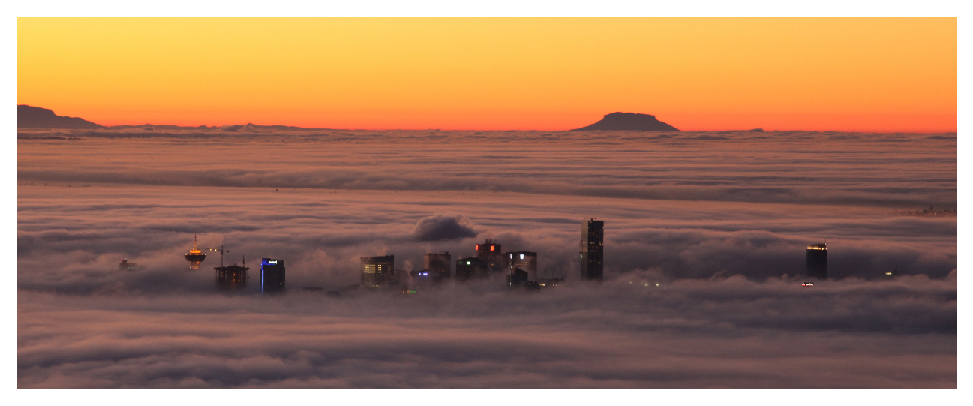
\includegraphics[width=\linewidth]{CypressView}
  \caption{In the Clouds: Vancouver from Cypress Mountain.}
  \label{fig:teaser}
}

%% Abstract section.
\abstract{
    360° videos provide an accessible form of immersive media for virtual reality (VR), yet their characteristic camera motion can induce motion sickness during viewing. Existing mitigation techniques often introduce visual distractions or distortions, potentially compromising immersion. Drawing on the theory of controllability in motion sickness, this paper investigates whether visualizing the capturing camera’s motion trajectory can mitigate motion sickness while preserving the immersive experience. We designed two interfaces that visualize camera trajectories in 360° VR: an overlay interface, which presents the trajectory within the viewer’s field of view, and a minimap interface, which provides a spatial overview of the trajectory. Across two user studies, we compared these interfaces with three conditions: unmodified 360° VR, a counter-optical-flow visualization, and a dynamic field-of-view technique. Results indicate that both trajectory-based interfaces effectively reduced motion sickness while preserving users’ sense of immersion. Our work demonstrates the potential of camera-trajectory visualization as a less intrusive approach to balancing motion sickness mitigation and immersion in 360° VR.
} % end of abstract

%% Keywords that describe your work. Will show as 'Index Terms' in journal
%% please capitalize first letter and insert punctuation after last keyword.
\keywords{Radiosity, global illumination, constant time.}

%% Copyright space is enabled by default as required by guidelines.
%% It is disabled by the 'review' option or via the following command:
% \nocopyrightspace

%%%%%%%%%%%%%%%%%%%%%%%%%%%%%%%%%%%%%%%%%%%%%%%%%%%%%%%%%%%%%%%%
%%%%%%%%%%%%%%%%%%%%%% START OF THE PAPER %%%%%%%%%%%%%%%%%%%%%%
%%%%%%%%%%%%%%%%%%%%%%%%%%%%%%%%%%%%%%%%%%%%%%%%%%%%%%%%%%%%%%%%%

\begin{document}

%% The ``\maketitle'' command must be the first command after the
%% ``\begin{document}'' command. It prepares and prints the title block.

%% the only exception to this rule is the \firstsection command
%\firstsection{Introduction}

\maketitle

\section{Introduction}

A coherent introduction could be structured into **6 paragraphs**, moving from the broad problem to the specific gap, theoretical grounding, proposed approach, and research contribution:

* **Paragraph 1 — 360° VR as accessible immersive media**

  * Introduce 360° videos as an increasingly accessible form of immersive content for VR.
  * Explain their advantages: users can freely explore the surrounding visual environment and experience recorded scenes from an immersive first-person perspective.
  * Highlight that unlike interactive VR experiences, 360° videos preserve real-world visual content while requiring relatively limited production and interaction infrastructure.
  * Transition to a key challenge: the camera motion embedded in 360° videos can cause motion sickness.

* **Paragraph 2 — Motion sickness in 360° video viewing**

  * Explain why camera motion in 360° videos can induce motion sickness, particularly when visually perceived motion is not accompanied by corresponding physical motion.
  * Briefly discuss symptoms and their negative effects on comfort, viewing duration, and the overall VR experience.
  * Emphasize that mitigating motion sickness is therefore important for making 360° VR more comfortable and usable.
  * Establish the tension between reducing sickness and preserving the immersive qualities that motivate users to watch 360° content in VR.

* **Paragraph 3 — Existing mitigation approaches and their limitations**

  * Review existing visual approaches for reducing motion sickness in VR/360° video.
  * Organize them around techniques such as **visual distraction**, **visual distortion**, **counter-optical-flow cues**, and **dynamic field-of-view manipulation**.
  * Explain that although these approaches can reduce users' exposure to provocative visual motion, they may obscure, distort, or restrict the visual scene.
  * Argue that such interventions can consequently reduce **visual immersion**, creating a trade-off between motion sickness mitigation and the quality of the immersive experience.
  * Identify the need for approaches that mitigate sickness **without substantially altering the visual content**.

* **Paragraph 4 — Controllability as a theoretical basis**

  * Introduce the **theory of controllability in motion sickness** as an alternative perspective for mitigation.
  * Explain that perceived controllability over visually induced motion can influence users' susceptibility to motion sickness.
  * In prerecorded 360° videos, viewers cannot control the physical motion of the capturing camera, making the camera's movement potentially unpredictable or difficult to anticipate.
  * Motivate the idea that explicitly communicating the **camera's motion trajectory** could provide users with information about upcoming or ongoing movement, thereby increasing their perceived controllability.
  * Position trajectory visualization as a way to address motion sickness through **additional information rather than visual distortion**.

* **Paragraph 5 — Proposed approach and research questions**

  * Introduce the proposed approach: visualizing the **capturing camera's motion trajectory** during 360° video viewing.
  * Describe the two interface designs:

    * **Overlay:** directly presents the camera trajectory within the user's view.
    * **Minimap:** presents the trajectory as a spatial overview, allowing users to understand camera movement from a broader perspective.
  * Explain the design rationale and how the two interfaces provide trajectory information through different spatial representations.
  * State that two user studies evaluate these interfaces against:

    * a baseline 360° VR condition without visual enhancement,
    * a counter-optical-flow visualization,
    * and a dynamic field-of-view technique.
  * Frame the investigation around two central questions: **(1) Can camera-trajectory visualization reduce motion sickness? (2) Can it do so while preserving users' sense of immersion?**

* **Paragraph 6 — Contributions**

  * Summarize the paper's contributions in **2–3 concrete points**:

    * **A design approach** for mitigating motion sickness in 360° VR through visualization of the capturing camera's motion trajectory, grounded in controllability theory.
    * **Two interface designs**, overlay and minimap, that operationalize trajectory visualization in different spatial representations.
    * **Empirical evidence from two user studies** comparing trajectory-based interfaces with existing visual mitigation approaches, demonstrating their ability to balance motion sickness mitigation and immersion.
  * Conclude by positioning the work as contributing to the design of **less intrusive motion-sickness mitigation techniques for immersive 360° video viewing**.

\section{Related work}
\section{Interfaces Leveraging Camera Trajectory Visualizations}
\section{Study 1}
\label{sec:study1}

Study 1 examined how different visual interventions affected visually induced motion sickness (VIMS), presence, and subjective preferences while participants viewed moving-camera 360$^\circ$ videos in VR. We used three approximately one-minute videos depicting walking, cycling, and driving. Each video was presented under four conditions: an unmodified \textit{Baseline}, \textit{Dynamic FOV}, our \textit{Minimap} trajectory visualization, and our \textit{Overlay Path} trajectory visualization. Thus, the study followed a 4 (Method) $\times$ 3 (Video) within-subjects design. Study 2 included \textit{Reverse Optical Flow} for direct comparison with our two trajectory-visualization techniques.

\subsection{Participants}

We recruited 36 participants. All participants completed all 12 experimental conditions (four methods $\times$ three videos), yielding 432 observations with no missing quantitative data. To reduce carryover of VIMS symptoms from one condition to the next, participants rested for 15 minutes between consecutive conditions; after every third condition, the washout period was extended to 30 minutes. 

\subsection{Study Design and Procedure}

Each participant viewed the walking, cycling, and driving videos under all four visualization conditions. Each exposure lasted approximately one minute and was followed by the study measures described below and the scheduled washout period. To reduce order effects, we counterbalanced the presentation order of the four visualization conditions using a balanced Latin square.


\subsection{Measures}
\label{subsec:study1-measures}

\paragraph{Simulator sickness.}
We assessed sickness using the 16-item Simulator Sickness Questionnaire (SSQ) and computed the Kennedy weighted scores for Total Severity (TSC), Nausea (N), Oculomotor discomfort (O), and Disorientation (D). Higher scores indicate more severe sickness symptoms. Besides, to ensure every participant understand the 16 questions correctly, we use the Vietnamese version of the original 16-item SSQ. 
% TODO: Add Kennedy et al. (1993) to References.bib and cite it here.

\paragraph{Immersion.}
We also assessed the participants' sense of immersion using a five-item, 7-point Likert questionnaire adapted from established measures of immersion in virtual environments. Responses ranged from 1 (strongly disagree) to 7 (strongly agree), with higher mean scores indicating stronger perceived immersion. 


\paragraph{Preference ranking and post-study interviews.}

After completing all 12 conditions, participants took part in a semi-structured interview about their VIMS experience and the three mitigation techniques. Questions focused on perceived sickness reduction, anticipation of camera motion, visual stability, attention demands, and trade-offs between comfort and presence. Participants also discussed specific usability issues, such as looking away from the scene to check the minimap, excessive attention drawn by the overlay path, and the restricted peripheral view caused by Dynamic FOV.

A subset of 13 participants (36.1\%) additionally ranked the four conditions from 1 (most preferred) to 4 (least preferred). Because rankings were available for only 13 of 36 participants, we treated them as exploratory descriptive evidence. Interview responses were analyzed thematically to help interpret differences between the mitigation techniques.

\subsection{Analysis}

For the SSQ scores and presence ratings, we conducted two-way repeated-measures ANOVAs with \textit{Method} (Baseline, Dynamic FOV, Minimap, Overlay Path) and \textit{Video} (Cycling, Walking, Driving) as within-subject factors. Greenhouse--Geisser corrections were applied to the repeated-measures $F$ tests. For the four SSQ outcomes, Holm corrections were applied across dependent variables within each effect family, and Bonferroni-adjusted pairwise comparisons were used for significant Method effects. We report generalized eta squared ($\eta_G^2$) as the effect size.

The SSQ residuals deviated from normality, primarily because of heavy tails rather than pronounced skewness. We therefore assessed robustness by repeating the SSQ analyses after excluding the three participants associated with extreme outliers. The significance pattern was unchanged across all combinations of SSQ effects and dependent variables, so the results below use the full sample ($N=36$).

\subsection{Results}
\label{subsec:study1-results}

\subsubsection{VIMS and SSQ}

We conducted a two-way repeated-measures ANOVA with Method and Video as within-subject factors. As summarized in Table~\ref{tab:study1-anova}, \textbf{Method significantly affected all four SSQ measures}, whereas neither Video nor the Method $\times$ Video interaction was significant. This indicates that the mitigation effects were broadly consistent across the walking, cycling, and driving videos.

\begin{table*}[t]
    \centering
    \caption{Repeated-measures ANOVA results for Study 1. Greenhouse--Geisser-corrected degrees of freedom are reported. Holm correction was applied across the four SSQ outcomes.}
    \label{tab:study1-anova}
    \small
    \begin{tabular}{lccccc}
        \toprule
        \textbf{Effect} & \textbf{TSC} & \textbf{Nausea} & \textbf{Oculomotor} & \textbf{Disorientation} & \textbf{Presence} \\
        \midrule

        Method &
        \textbf{$F=9.02$, $p<.001$} &
        \textbf{$F=7.37$, $p<.001$} &
        \textbf{$F=8.63$, $p<.001$} &
        \textbf{$F=6.98$, $p<.001$} &
        \textbf{$F=13.64$, $p<.001$} \\

        Video &
        $p=.230$ &
        $p=.229$ &
        $p=.084$ &
        $p=.410$ &
        $p=.450$ \\

        Method $\times$ Video &
        $p=.535$ &
        $p=.570$ &
        $p=.392$ &
        $p=.642$ &
        $p=.109$ \\

        \bottomrule
    \end{tabular}
\end{table*}

Table~\ref{tab:study1-method-summary} summarizes the main differences between visualization methods. Lower SSQ scores indicate less VIMS, while higher Presence scores indicate a stronger sense of presence.

\begin{table*}[t]
    \centering
    \caption{Main quantitative results by visualization method, collapsed across video type. SSQ and Presence values are means $\pm$ SD. Percentage reductions in TSC are relative to Baseline.}
    \label{tab:study1-method-summary}
    \small
    \begin{tabular}{lccccc}
        \toprule
        \textbf{Method}
        & \textbf{TSC}
        & \textbf{TSC reduction}
        & \textbf{Nausea}
        & \textbf{Disorientation}
        & \textbf{Presence} \\
        \midrule

        Baseline
        & $71.6 \pm 47.6$
        & --
        & $39.5 \pm 30.8$
        & $93.1 \pm 66.7$
        & \textbf{$4.79 \pm 0.94$} \\

        Dynamic FOV
        & \textbf{$48.3 \pm 38.7$}
        & \textbf{33\%}
        & \textbf{$26.6 \pm 26.4$}
        & \textbf{$62.4 \pm 50.9$}
        & $3.92 \pm 1.33$ \\

        Minimap
        & $55.5 \pm 38.0$
        & 22\%
        & $29.2 \pm 25.2$
        & $72.4 \pm 57.1$
        & \textbf{$4.53 \pm 1.00$} \\

        Overlay Path
        & $56.7 \pm 36.3$
        & 21\%
        & $30.4 \pm 22.1$
        & $73.9 \pm 54.0$
        & $4.41 \pm 1.02$ \\

        \bottomrule
    \end{tabular}
\end{table*}

\paragraph{Dynamic FOV.}
Dynamic FOV produced the \textbf{largest numerical reduction in VIMS}, reducing TSC by approximately 33\% relative to Baseline. However, it did not significantly outperform Minimap or Overlay Path on any SSQ measure.

\paragraph{Minimap.}
Minimap reduced TSC by approximately 22\% while maintaining the \textbf{highest Presence score among the three mitigation methods}.

\paragraph{Overlay Path.}
Overlay Path reduced TSC by approximately 21\%. Its reductions relative to Baseline were significant for TSC, Nausea, and Oculomotor discomfort, while the reduction in Disorientation did not reach significance after Bonferroni correction ($p=.0734$).

% ------------------------------------------------------------
% FIGURE PLACEHOLDER: SSQ
% Export the SSQ grouped bar chart as:
% figures/study1_ssq_by_method.png
% ------------------------------------------------------------

\begin{figure*}[t]
    \centering
    \IfFileExists{figures/study1_ssq_by_method.png}{
        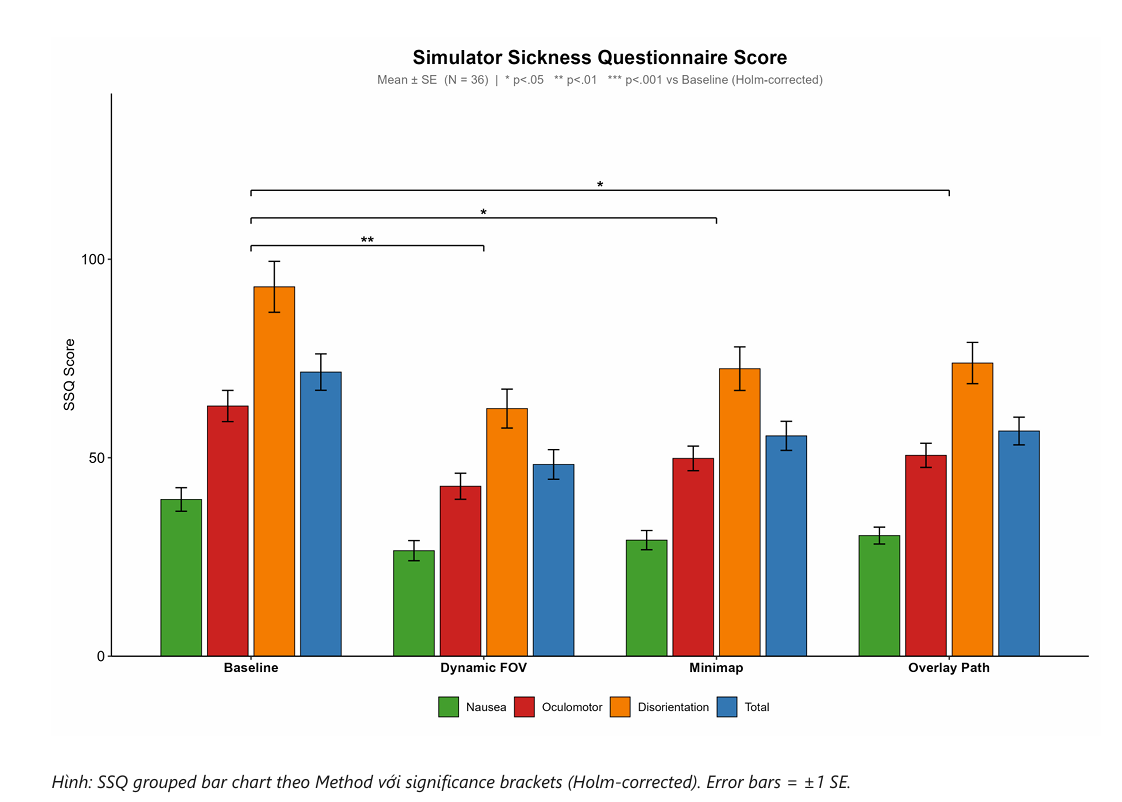
\includegraphics[width=0.88\textwidth]
        {figures/study1_ssq_by_method.png}
    }{}
    \caption{Simulator Sickness Questionnaire scores across visualization methods. Lower scores indicate less VIMS. Error bars show $\pm1$ SE; brackets indicate significant pairwise comparisons.}
    \label{fig:study1-ssq-method}
\end{figure*}


\subsubsection{Presence and the VIMS--Presence Trade-off}

The pattern for Presence differed from the SSQ results. Table~\ref{tab:study1-presence-pairwise} highlights the pairwise comparisons most relevant to the VIMS--Presence trade-off.

\begin{table}[t]
    \centering
    \caption{Key Bonferroni-adjusted pairwise comparisons for Presence.}
    \label{tab:study1-presence-pairwise}
    \small
    \begin{tabular}{lcc}
        \toprule
        \textbf{Comparison} & $\boldsymbol{\Delta}$ \textbf{Presence} & \textbf{$p$} \\
        \midrule
        Baseline -- Dynamic FOV & +0.861 & \textbf{.0006} \\
        Baseline -- Minimap & +0.254 & .1984 \\
        Baseline -- Overlay Path & +0.372 & \textbf{.0093} \\
        Dynamic FOV -- Minimap & -0.607 & \textbf{.0022} \\
        Dynamic FOV -- Overlay Path & -0.489 & \textbf{.0101} \\
        Minimap -- Overlay Path & +0.119 & 1.000 \\
        \bottomrule
    \end{tabular}
\end{table}

\paragraph{Dynamic FOV.}
Although Dynamic FOV achieved the largest numerical VIMS reduction, it also produced the \textbf{lowest Presence score} ($M=3.92$), significantly below the other three conditions.

\paragraph{Minimap.}
Minimap preserved Presence most effectively: its score did not significantly differ from Baseline ($p=.1984$).

\paragraph{Overlay Path.}
Overlay Path produced a smaller but significant reduction in Presence relative to Baseline ($p=.0093$).

These results indicate a clear \textbf{VIMS--Presence trade-off}: stronger sickness mitigation does not necessarily correspond to a better overall viewing experience.

% ------------------------------------------------------------
% FIGURE PLACEHOLDER: PRESENCE
% Export the Presence boxplot as:
% figures/study1_presence_by_method.png
% ------------------------------------------------------------

\begin{figure}[t]
    \centering
    \IfFileExists{figures/study1_presence_by_method.png}{
        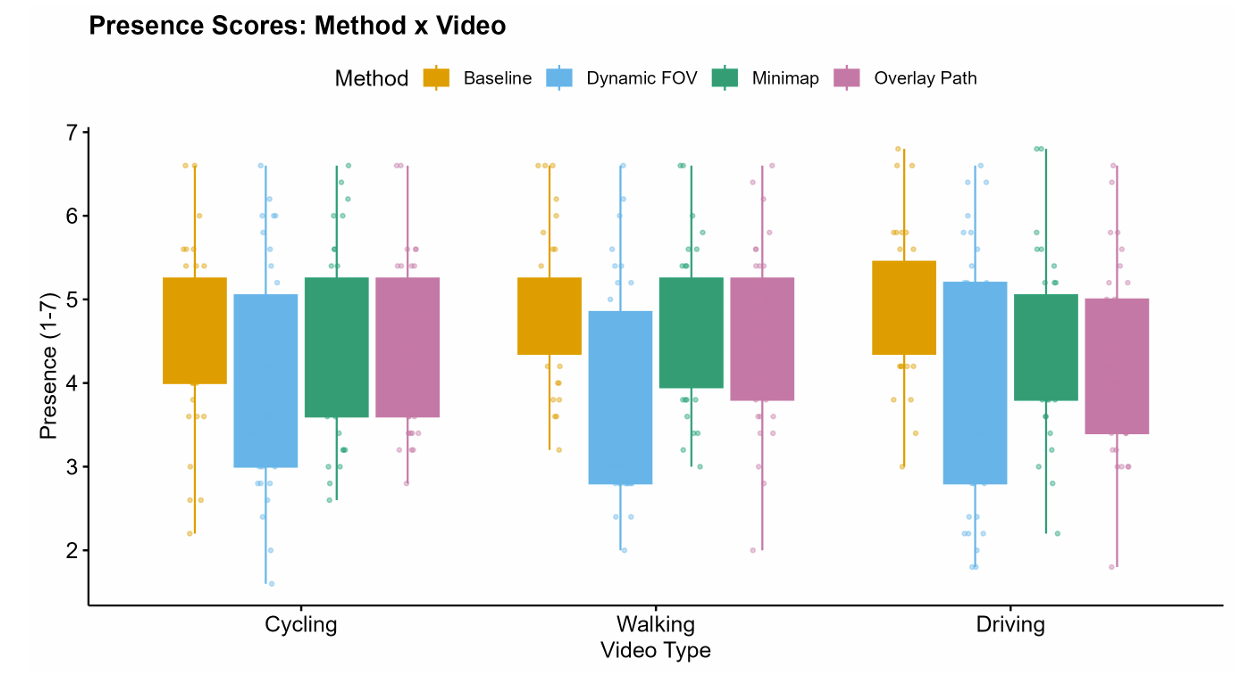
\includegraphics[width=\columnwidth]
        {figures/study1_presence_by_method.png}
    }{}
    \caption{Presence ratings across visualization methods and video types. Higher values indicate stronger perceived presence.}
    \label{fig:study1-presence}
\end{figure}


\subsubsection{Qualitative Feedback}

The interviews further explain the differences between the three mitigation methods. Table~\ref{tab:study1-mixed-methods} summarizes the main qualitative observations together with the corresponding quantitative results.

\begin{table*}[t]
    \centering
    \caption{Integration of quantitative and qualitative findings.}
    \label{tab:study1-mixed-methods}
    \small
    \begin{tabular}{
        p{0.14\textwidth}
        p{0.34\textwidth}
        p{0.44\textwidth}}
        \toprule

        \textbf{Method}
        & \textbf{Quantitative result}
        & \textbf{Interview feedback} \\

        \midrule

        Minimap
        &
        TSC reduced by 22\%; Presence remained closest to Baseline ($p=.1984$).
        &
        Familiar and stable for some participants, but its small size and low position required users to look away from the main scene, producing additional attention cost. \\

        Overlay Path
        &
        TSC reduced by 21\%; small Presence reduction relative to Baseline ($p=.0093$).
        &
        Helped some participants anticipate the camera trajectory. However, visual distraction and difficulty initially understanding the function of the path could interfere with the experience. \\

        Dynamic FOV
        &
        \textbf{Largest TSC reduction (33\%)}, but \textbf{lowest Presence} ($M=3.92$) and highest Presence variability ($SD=1.33$).
        &
        Highly polarized. Some participants reported that reducing peripheral motion helped alleviate discomfort, while others disliked the restricted peripheral view. \\

        \bottomrule
    \end{tabular}
\end{table*}

Overall, the interviews suggest that the effectiveness of each technique depends not only on sickness reduction, but also on how the visual aid affects attention, and even the exposure duration to the 360 video: \textbf{some participants even suggest that for longer 360 videos, they would trade immersion with VIMS reduction}. 


\subsubsection{Exploratory Preference Ranking}

Because preference rankings were available for only 13 of the 36 participants (36.1\%), these results are treated as exploratory. However in study 2, a complete reference ranking is available. 

\begin{table}[t]
    \centering
    \caption{Exploratory preference ranking. Lower mean rank indicates stronger preference. First- and last-choice counts are tie-adjusted.}
    \label{tab:study1-preference}
    \small
    \begin{tabular}{lcccc}
        \toprule
        \textbf{Method}
        & \textbf{Mean rank}
        & \textbf{Borda}
        & \textbf{First}
        & \textbf{Last} \\
        \midrule

        \textbf{Overlay Path} & \textbf{2.04} & \textbf{38.5} & 4.0 & \textbf{0.5} \\
        Minimap & 2.42 & 33.5 & 1.0 & 1.0 \\
        Dynamic FOV & 2.73 & 29.5 & \textbf{5.0} & \textbf{6.5} \\
        Baseline & 2.81 & 28.5 & 3.0 & 5.0 \\

        \bottomrule
    \end{tabular}
\end{table}

\paragraph{Overlay Path.}
Overlay Path had the \textbf{best overall mean rank and Borda score} and was almost never ranked last.

\paragraph{Dynamic FOV.}
Dynamic FOV again showed the strongest polarization: it received both the \textbf{largest number of first-choice rankings} and the \textbf{largest number of last-choice rankings}.

% OPTIONAL FIGURE
% figures/study1_preference_rank.png
%
% \begin{figure}[t]
%     \centering
%     \includegraphics[width=\columnwidth]
%     {figures/study1_preference_rank.png}
%     \caption{Mean preference rank across visualization methods.
%     Lower values indicate stronger preference.}
%     \label{fig:study1-preference-rank}
% \end{figure}


\subsubsection{Study 1 Summary}

Taken together, Study 1 shows that all three visualization techniques reduced VIMS relative to the unmodified Baseline, while their effects remained consistent across the three video types. \textbf{Dynamic FOV} provided the greatest numerical sickness reduction but substantially reduced Presence and produced polarized responses. \textbf{Minimap} provided the strongest quantitative balance between VIMS mitigation and Presence preservation. \textbf{Overlay Path} achieved a similar VIMS reduction while receiving the strongest exploratory preference ranking, although interview feedback highlighted the importance of clear and visually stable implementation.


% Study 2. Numbers come from results/study2/study2_results.txt,
% results/study2/trajectory/study2_trajectory_results.txt and
% results/study2/preference/study2_preference_results.txt.

\section{Study 2}
\label{sec:study2}

Study~1 showed that both trajectory visualizations reduced VIMS relative to
unmodified 360$^\circ$ video while costing less Presence than Dynamic FOV.
However, Study~1 compared them with only one other mitigation technique and
measured sickness only after each trial. Study~2 therefore compared our
\textit{Minimap} and \textit{Overlay Path} interfaces with \textit{Reverse
Optical Flow} (ROF), a counter-optical-flow visualization. We treated Minimap
and Overlay Path as the \emph{trajectory-based} interfaces and ROF as the
\emph{non-trajectory} comparison, and asked: \textbf{are trajectory-based
interfaces as effective as ROF at reducing VIMS, while being less intrusive?}
Study~2 also measured sickness both before and after every trial, and
collected a complete preference ranking and interview from every participant.

\subsection{Participants}

We recruited 36 participants. % TODO: age range, gender, and whether any also took part in Study 1.
Nineteen had used a VR headset before and 17 had not. All participants
completed all nine experimental conditions (three methods $\times$ three
videos), yielding 324 trials and 648 SSQ administrations with no missing data.

\subsection{Study Design and Procedure}

Study~2 followed a 3 (\textit{Method}: ROF, Minimap, Overlay Path) $\times$ 3
(\textit{Video}: Walking, Cycling, Driving) within-subjects design. Unlike
Study~1, it had \textbf{no Baseline condition}, so all comparisons are between
mitigation techniques. Each participant experienced the three methods in
separate blocks, and each block contained all three videos. Method order was
fully counterbalanced: each of the six possible orders was assigned to six
participants. Video order within blocks was counterbalanced so that each video
appeared equally often in each position. Participants completed the SSQ
immediately before each video, and the SSQ and the Presence questionnaire
immediately after it. The median interval between finishing one trial and
starting the next was 6.3 minutes (IQR 5.1--7.3). After all nine trials,
participants ranked the three methods and took part in a short interview.

\subsection{Measures}

\paragraph{Simulator sickness.}
We used the same Vietnamese version of the 16-item SSQ and the same Kennedy
weighted scores (TSC, N, O, D) as in Study~1, but administered the
questionnaire both before and after every trial. Our main outcome was the
change score $\Delta = \text{post} - \text{pre}$, where positive values mean
that symptoms increased during viewing. The pre-trial scores also let us check
that participants started each condition at a similar level of sickness.

\paragraph{Immersion.}
Participants completed the same five-item, 7-point presence questionnaire as in
Study~1 after every trial (Cronbach's $\alpha = .78$).

\paragraph{Preference ranking and post-study interviews.}
After all nine trials, every participant ranked the three methods from 1 (best)
to 3 by how well each balanced immersion and VIMS mitigation, and explained the
ranking in a semi-structured interview. Later participants were also asked
which method best reduced their sickness (21 named one method) and which felt
most realistic (26 named one method). We coded the interview notes with a
codebook of eleven codes in three families: \emph{perceived sickness},
\emph{perceived realism}, and \emph{interface experience} (occlusion,
distraction, glance cost, route anticipation, timing, visual noise, visibility,
familiarity, and agency). Each code was counted at most once per participant
and method, so all counts below are numbers of participants.

To address intrusiveness, we counted a \emph{recorded intrusiveness-related
complaint} when a participant criticized a method for blocking the scene
(occlusion), drawing attention away from it (distraction), requiring gaze
shifts (glance cost), or producing flicker or visual clutter (visual noise).
Participants were not asked directly whether a method was intrusive, so this
measure counts unprompted complaints; a method without complaints is not
thereby shown to be unobtrusive.

\subsection{Analysis}

For the SSQ, we conducted 2 (\textit{Time}: pre, post) $\times$ 3
(\textit{Method}) $\times$ 3 (\textit{Video}) repeated-measures ANOVAs.
The \textit{Time} $\times$ \textit{Method} interaction is the effect of
interest, because it tests whether the methods differed in how much sickness
increased during viewing. As in Study~1, we applied Greenhouse--Geisser
corrections, Holm corrections across the four SSQ outcomes, and report
$\eta^2_G$. Presence was analyzed with a 3 $\times$ 3 repeated-measures ANOVA.

To compare the trajectory-based interfaces with ROF, we computed for each
participant the difference between their mean $\Delta$TSC under Minimap and
Overlay Path and their $\Delta$TSC under ROF (contrast weights
$-1, \frac{1}{2}, \frac{1}{2}$). Because the question is whether the
trajectory-based interfaces are \emph{as effective as} ROF, we used a
\textbf{non-inferiority test} (one-sided $\alpha = .05$) with a margin of
$+5$ TSC points: the trajectory-based interfaces are non-inferior if the upper
limit of the 90\% confidence interval of the difference lies below $+5$. The
margin is one third of the smallest reduction relative to Baseline in Study~1
(14.9 TSC points, Overlay Path), so a non-inferior method keeps at least
two-thirds of that benefit. We checked the result with a mixed-effects model on
all 324 trials, a participant bootstrap, and separate tests for each
trajectory-based interface.

For intrusiveness, we computed for each participant the difference between
whether they complained about ROF (0 or 1) and the mean of the same indicator
for Minimap and Overlay Path. We tested whether this difference was positive
with an exact permutation test that enumerates every assignment of the three
method labels within each participant. Answering the research question in the
affirmative required both the non-inferiority test and the intrusiveness test
to be significant; because both must succeed, no further $\alpha$ adjustment is
needed.

For the ranking, we used a Friedman test with Kendall's $W$, and a
Plackett--Luce model in which Minimap and Overlay Path share one preference
parameter.

The SSQ change scores were zero-inflated and heavy-tailed. Rank-transformed
ANOVAs, Friedman tests, bootstrap confidence intervals, and a mixed model
excluding extreme values all led to the same conclusions, so we report the
parametric results below.

\subsection{Results}

\subsubsection{VIMS and SSQ}

Table~\ref{tab:s2-anova} summarizes the ANOVA results and
Table~\ref{tab:s2-means} the scores for each method. \textbf{Viewing increased
sickness under every method}: \textit{Time} was significant for all four SSQ
outcomes, and TSC rose from 9.55 before to 17.98 after viewing (+8.44, 95\% CI
[5.27, 11.61], $d_z = 0.90$). \textbf{The method did not affect how much
sickness increased}: the \textit{Time} $\times$ \textit{Method} interaction was
not significant for any SSQ outcome (all $F \le 0.78$, uncorrected
$p \ge .44$, $\eta^2_G \le .001$). As Figure~\ref{fig:s2-prepost} shows, TSC
increased by 9.00 points with ROF, 9.07 with Minimap, and 7.24 with Overlay
Path. Participants started each method at a similar level (pre-trial TSC 9.90,
9.38, and 9.35; all $p \ge .77$), so these differences reflect what happened
during viewing.

The \textbf{video type} mattered more than the method. The \textit{Time}
$\times$ \textit{Video} interaction was significant for TSC, Oculomotor
discomfort, and Disorientation: the Walking video increased TSC by 13.09
points, roughly 2.4 times the increase for Driving (5.44) and nearly twice that
for Cycling (6.79). Walking differed from both other videos (Bonferroni
$p \le .003$), whereas Cycling and Driving did not differ. The three-way
interaction was not significant, so no method was better suited to a
particular video.

Symptoms partly carried over between trials: the post-trial TSC of one trial
predicted the pre-trial TSC of the next ($b = 0.39$, $p < .001$). Because
method order was fully counterbalanced, this carryover adds noise but does not
favor any method.

\begin{table*}[t]
  \caption{Repeated-measures ANOVA results for Study~2. SSQ outcomes were
  analyzed with a 2 (Time) $\times$ 3 (Method) $\times$ 3 (Video) ANOVA;
  Presence, measured after viewing only, with a 3 (Method) $\times$ 3 (Video)
  ANOVA. $F$ values are reported for significant effects;
  Greenhouse--Geisser corrections were applied, and $p$ values for the SSQ
  outcomes are Holm-corrected across the four outcomes. Time: $df = 1, 35$.}
  \label{tab:s2-anova}
  \centering
  \footnotesize
  \begin{tabular}{lccccc}
    \toprule
    \textbf{Effect} & \textbf{TSC} & \textbf{Nausea} & \textbf{Oculomotor} & \textbf{Disorientation} & \textbf{Presence} \\
    \midrule
    Time                          & $F = 29.15$, $p < .001$ & $F = 11.08$, $p = .002$ & $F = 23.97$, $p < .001$ & $F = 28.64$, $p < .001$ & -- \\
    Method                        & $p = 1.000$ & $p = 1.000$ & $p = 1.000$ & $p = 1.000$ & $p = .758$ \\
    Video                         & $p = .101$ & $p = .253$ & $F = 5.72$, $p = .021$ & $p = .192$ & $p = .311$ \\
    \textbf{Time $\times$ Method} & $p = 1.000$ & $p = 1.000$ & $p = 1.000$ & $p = 1.000$ & -- \\
    Time $\times$ Video           & $F = 7.73$, $p = .004$ & $p = .060$ & $F = 9.61$, $p = .001$ & $F = 6.91$, $p = .008$ & -- \\
    Method $\times$ Video         & $p = 1.000$ & $p = 1.000$ & $p = 1.000$ & $p = 1.000$ & $p = .568$ \\
    Time $\times$ Method $\times$ Video & $p = 1.000$ & $p = 1.000$ & $p = 1.000$ & $p = 1.000$ & -- \\
    \bottomrule
  \end{tabular}
\end{table*}

\begin{table*}[t]
  \caption{Main quantitative results of Study~2 by method, collapsed across
  video type (participant means $\pm$ SD, $n = 36$). $\Delta$ is the
  post-minus-pre change; positive values mean symptoms increased during
  viewing.}
  \label{tab:s2-means}
  \centering
  \footnotesize
  \begin{tabular}{lccccccc}
    \toprule
    \textbf{Method} & \textbf{Pre TSC} & \textbf{Post TSC} & \textbf{$\Delta$TSC} & \textbf{$\Delta$Nausea} & \textbf{$\Delta$Oculomotor} & \textbf{$\Delta$Disorientation} & \textbf{Presence} \\
    \midrule
    ROF          & $9.90 \pm 18.65$ & $18.91 \pm 21.18$ & $9.00 \pm 9.56$  & $3.97 \pm 6.24$ & $7.65 \pm 9.86$  & $13.66 \pm 15.45$ & $5.10 \pm 1.04$ \\
    Minimap      & $9.38 \pm 15.02$ & $18.46 \pm 20.51$ & $9.07 \pm 11.39$ & $3.27 \pm 9.33$ & $8.91 \pm 11.83$ & $12.63 \pm 16.32$ & $5.12 \pm 1.05$ \\
    Overlay Path & $9.35 \pm 19.45$ & $16.59 \pm 21.59$ & $7.24 \pm 12.60$ & $2.56 \pm 7.93$ & $6.67 \pm 12.28$ & $10.96 \pm 17.22$ & $5.04 \pm 1.06$ \\
    \bottomrule
  \end{tabular}
\end{table*}

\begin{figure*}[t]
  \centering
  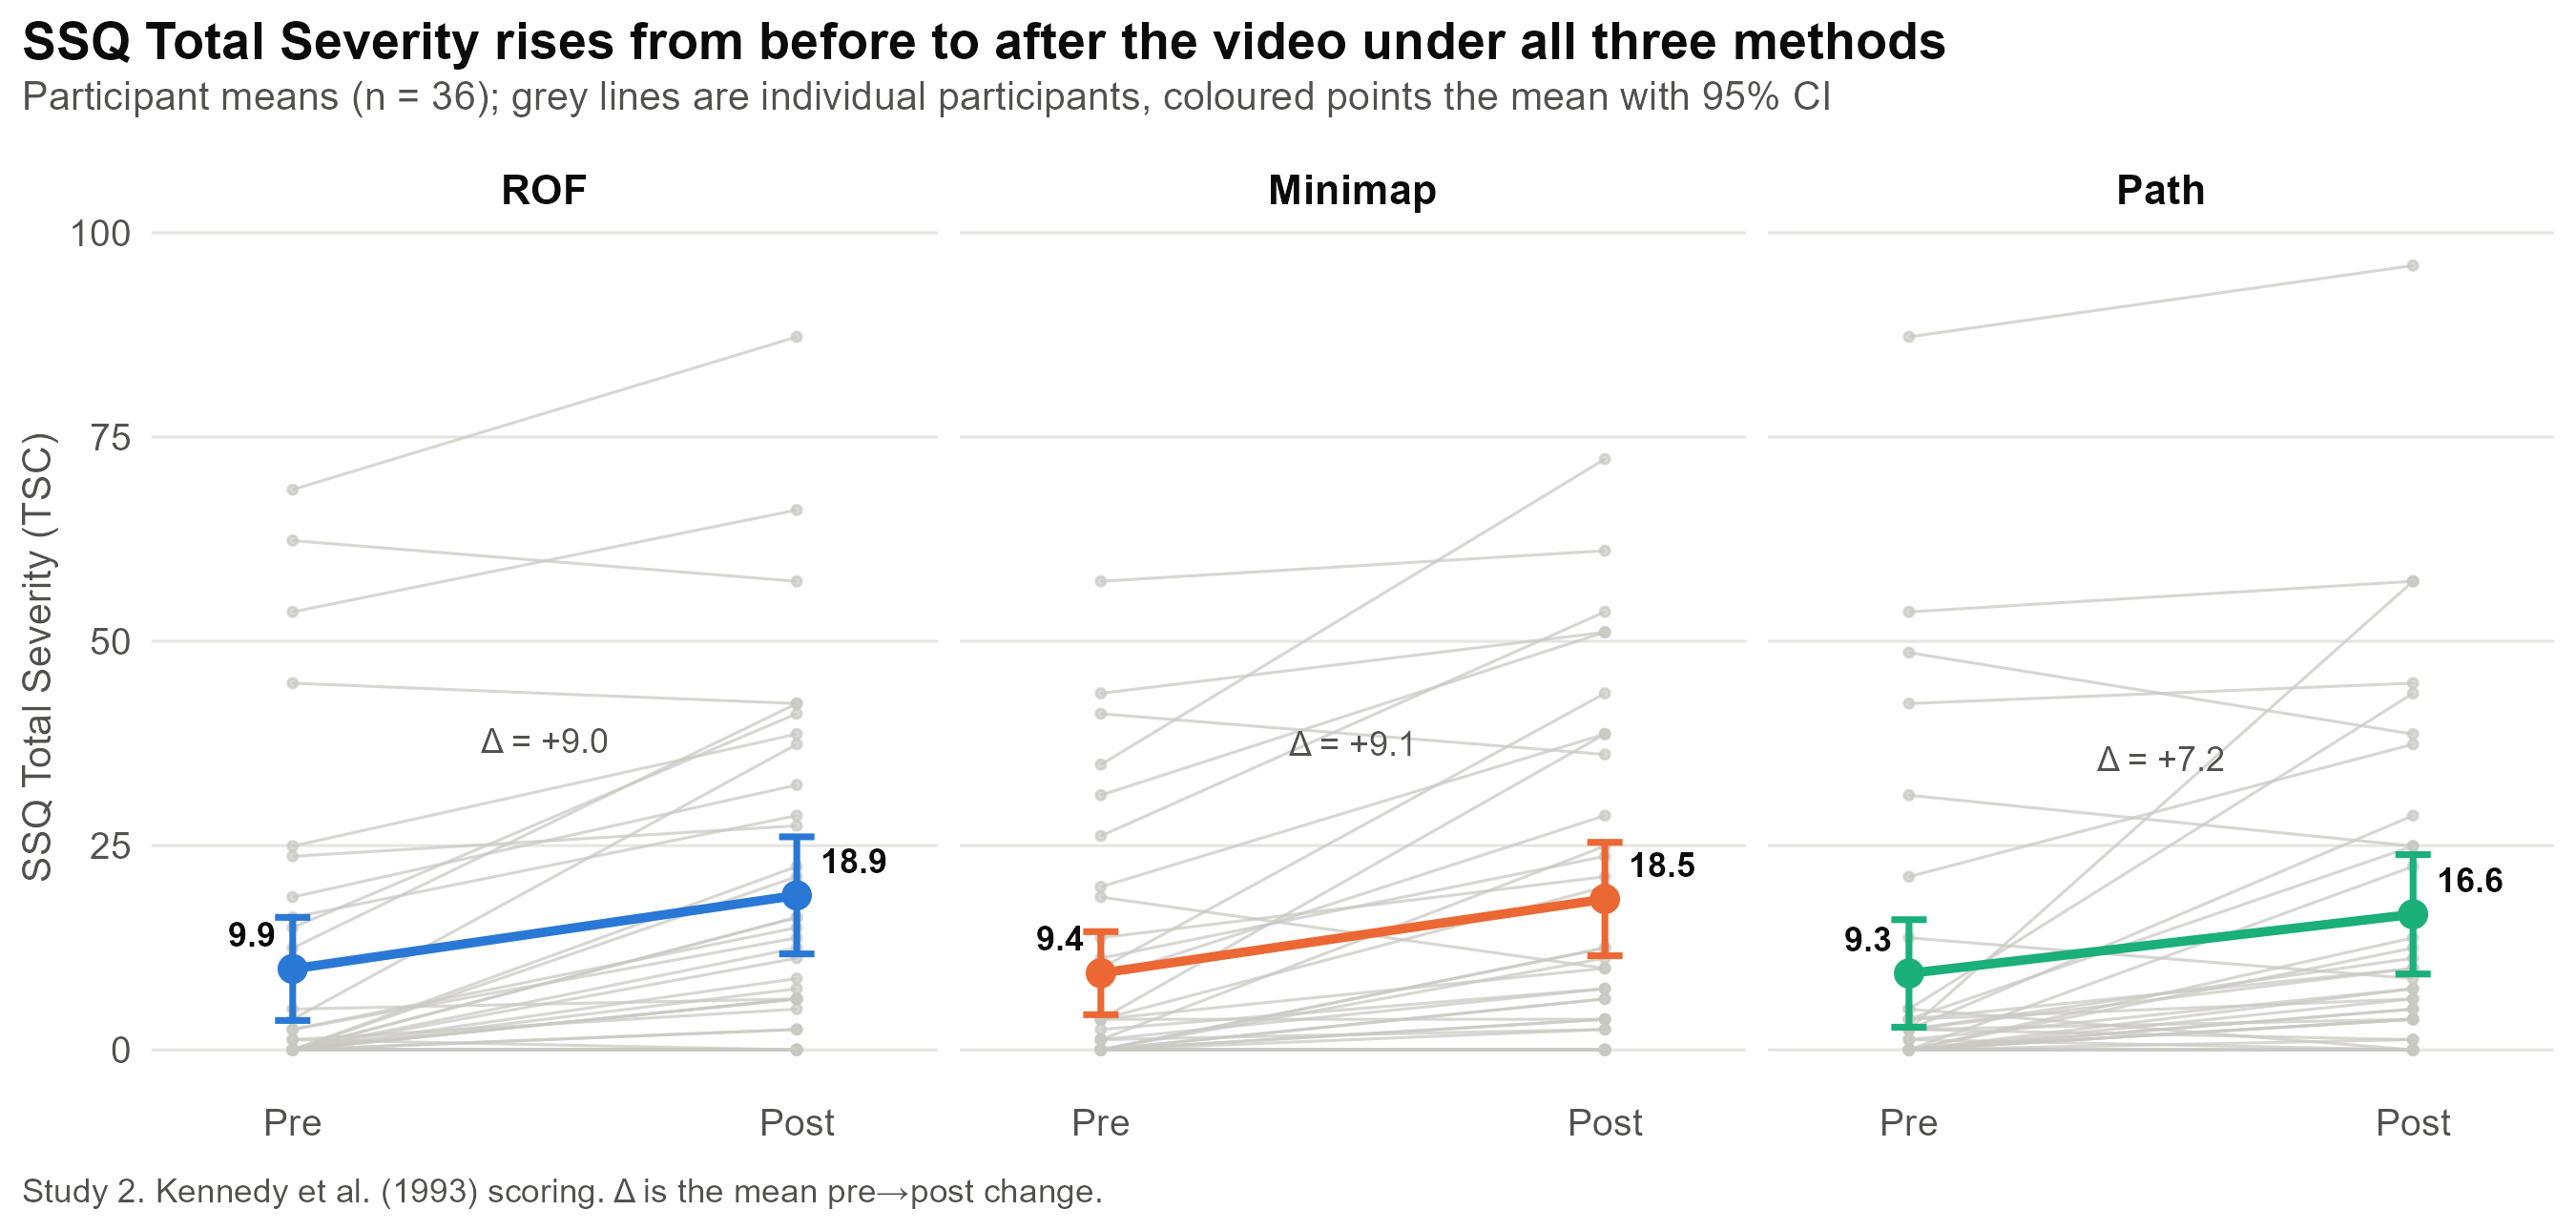
\includegraphics[width=\textwidth]{figures/study2_pre_post_tsc.png}
  \caption{SSQ Total Severity before and after each video in Study~2. Grey
  lines are individual participants (means over the three videos); colored
  points show the mean with 95\% CI. Sickness rose by a similar amount under
  all three methods.}
  \label{fig:s2-prepost}
\end{figure*}

\subsubsection{Are Trajectory-Based Interfaces as Effective as ROF?}

Table~\ref{tab:s2-ni} and Figure~\ref{fig:s2-ni} show the non-inferiority
results. \textbf{The trajectory-based interfaces were non-inferior to ROF in
measured VIMS.} On average, TSC increased 0.85 points \emph{less} with the
trajectory-based interfaces than with ROF (90\% CI [$-2.54$, 0.84]). The upper
limit was well below the $+5$ margin ($p < .001$), and the result held in the
mixed-effects model (upper limit 2.41) and the bootstrap (0.76).
\textbf{Both interfaces were individually non-inferior}: the upper limit was
2.71 for Minimap and 0.69 for Overlay Path (Holm-corrected $p \le .002$). The
difference also lay within $\pm 5$ points in a two-sided equivalence test, so
the trajectory-based interfaces were not meaningfully \emph{better} than ROF
either. No SSQ subscale differed between the groups (all Holm-corrected
$p \ge .83$), and the contrast did not vary by video
($F(1.73, 60.71) = 0.82$, $p = .43$).

Because Study~2 has no Baseline, this result shows that the trajectory-based
interfaces were about as effective as ROF; it does not show that any of the
three methods reduced VIMS relative to unmodified 360$^\circ$ video.

\paragraph{Comparison with Study 1.}
Applying the same contrast to Study~1, with Dynamic FOV as the non-trajectory
comparison, did not establish non-inferiority: post-trial TSC was 7.8 points
higher with the trajectory-based interfaces than with Dynamic FOV (95\% CI
[$-0.9$, 16.5]). This interval includes both zero and the margin, so the
comparison is inconclusive. In Study~1, the trajectory-based interfaces still
reduced TSC by 15.5 points relative to Baseline (95\% CI [6.5, 24.4]) and
produced higher Presence than Dynamic FOV ($+0.55$, 95\% CI [0.26, 0.84]).

\begin{table}[t]
  \caption{Non-inferiority of the trajectory-based interfaces. Difference in
  TSC points (trajectory minus comparison; positive = more sickness).
  Non-inferior when the upper limit of the 90\% CI is below the $+5$ margin.
  Study~2 uses the pre-to-post change; Study~1 uses post-trial TSC.}
  \label{tab:s2-ni}
  \centering
  \footnotesize
  \begin{tabular}{lccc}
    \toprule
    \textbf{Comparison} & \textbf{Difference} & \textbf{90\% CI} & \textbf{Non-inferior} \\
    \midrule
    \multicolumn{4}{l}{\textit{Study 2 (vs ROF)}} \\
    Trajectory (pooled) & $-0.85$ & [$-2.54$, 0.84] & \textbf{yes} \\
    Minimap             & $+0.07$ & [$-2.57$, 2.71] & \textbf{yes} \\
    Overlay Path        & $-1.77$ & [$-4.22$, 0.69] & \textbf{yes} \\
    \midrule
    \multicolumn{4}{l}{\textit{Study 1 (vs Dynamic FOV)}} \\
    Trajectory (pooled) & $+7.81$ & [0.54, 15.08]   & no \\
    Minimap             & $+7.20$ & [0.16, 14.25]   & no \\
    Overlay Path        & $+8.42$ & [$-0.08$, 16.91] & no \\
    \bottomrule
  \end{tabular}
\end{table}

\begin{figure*}[t]
  \centering
  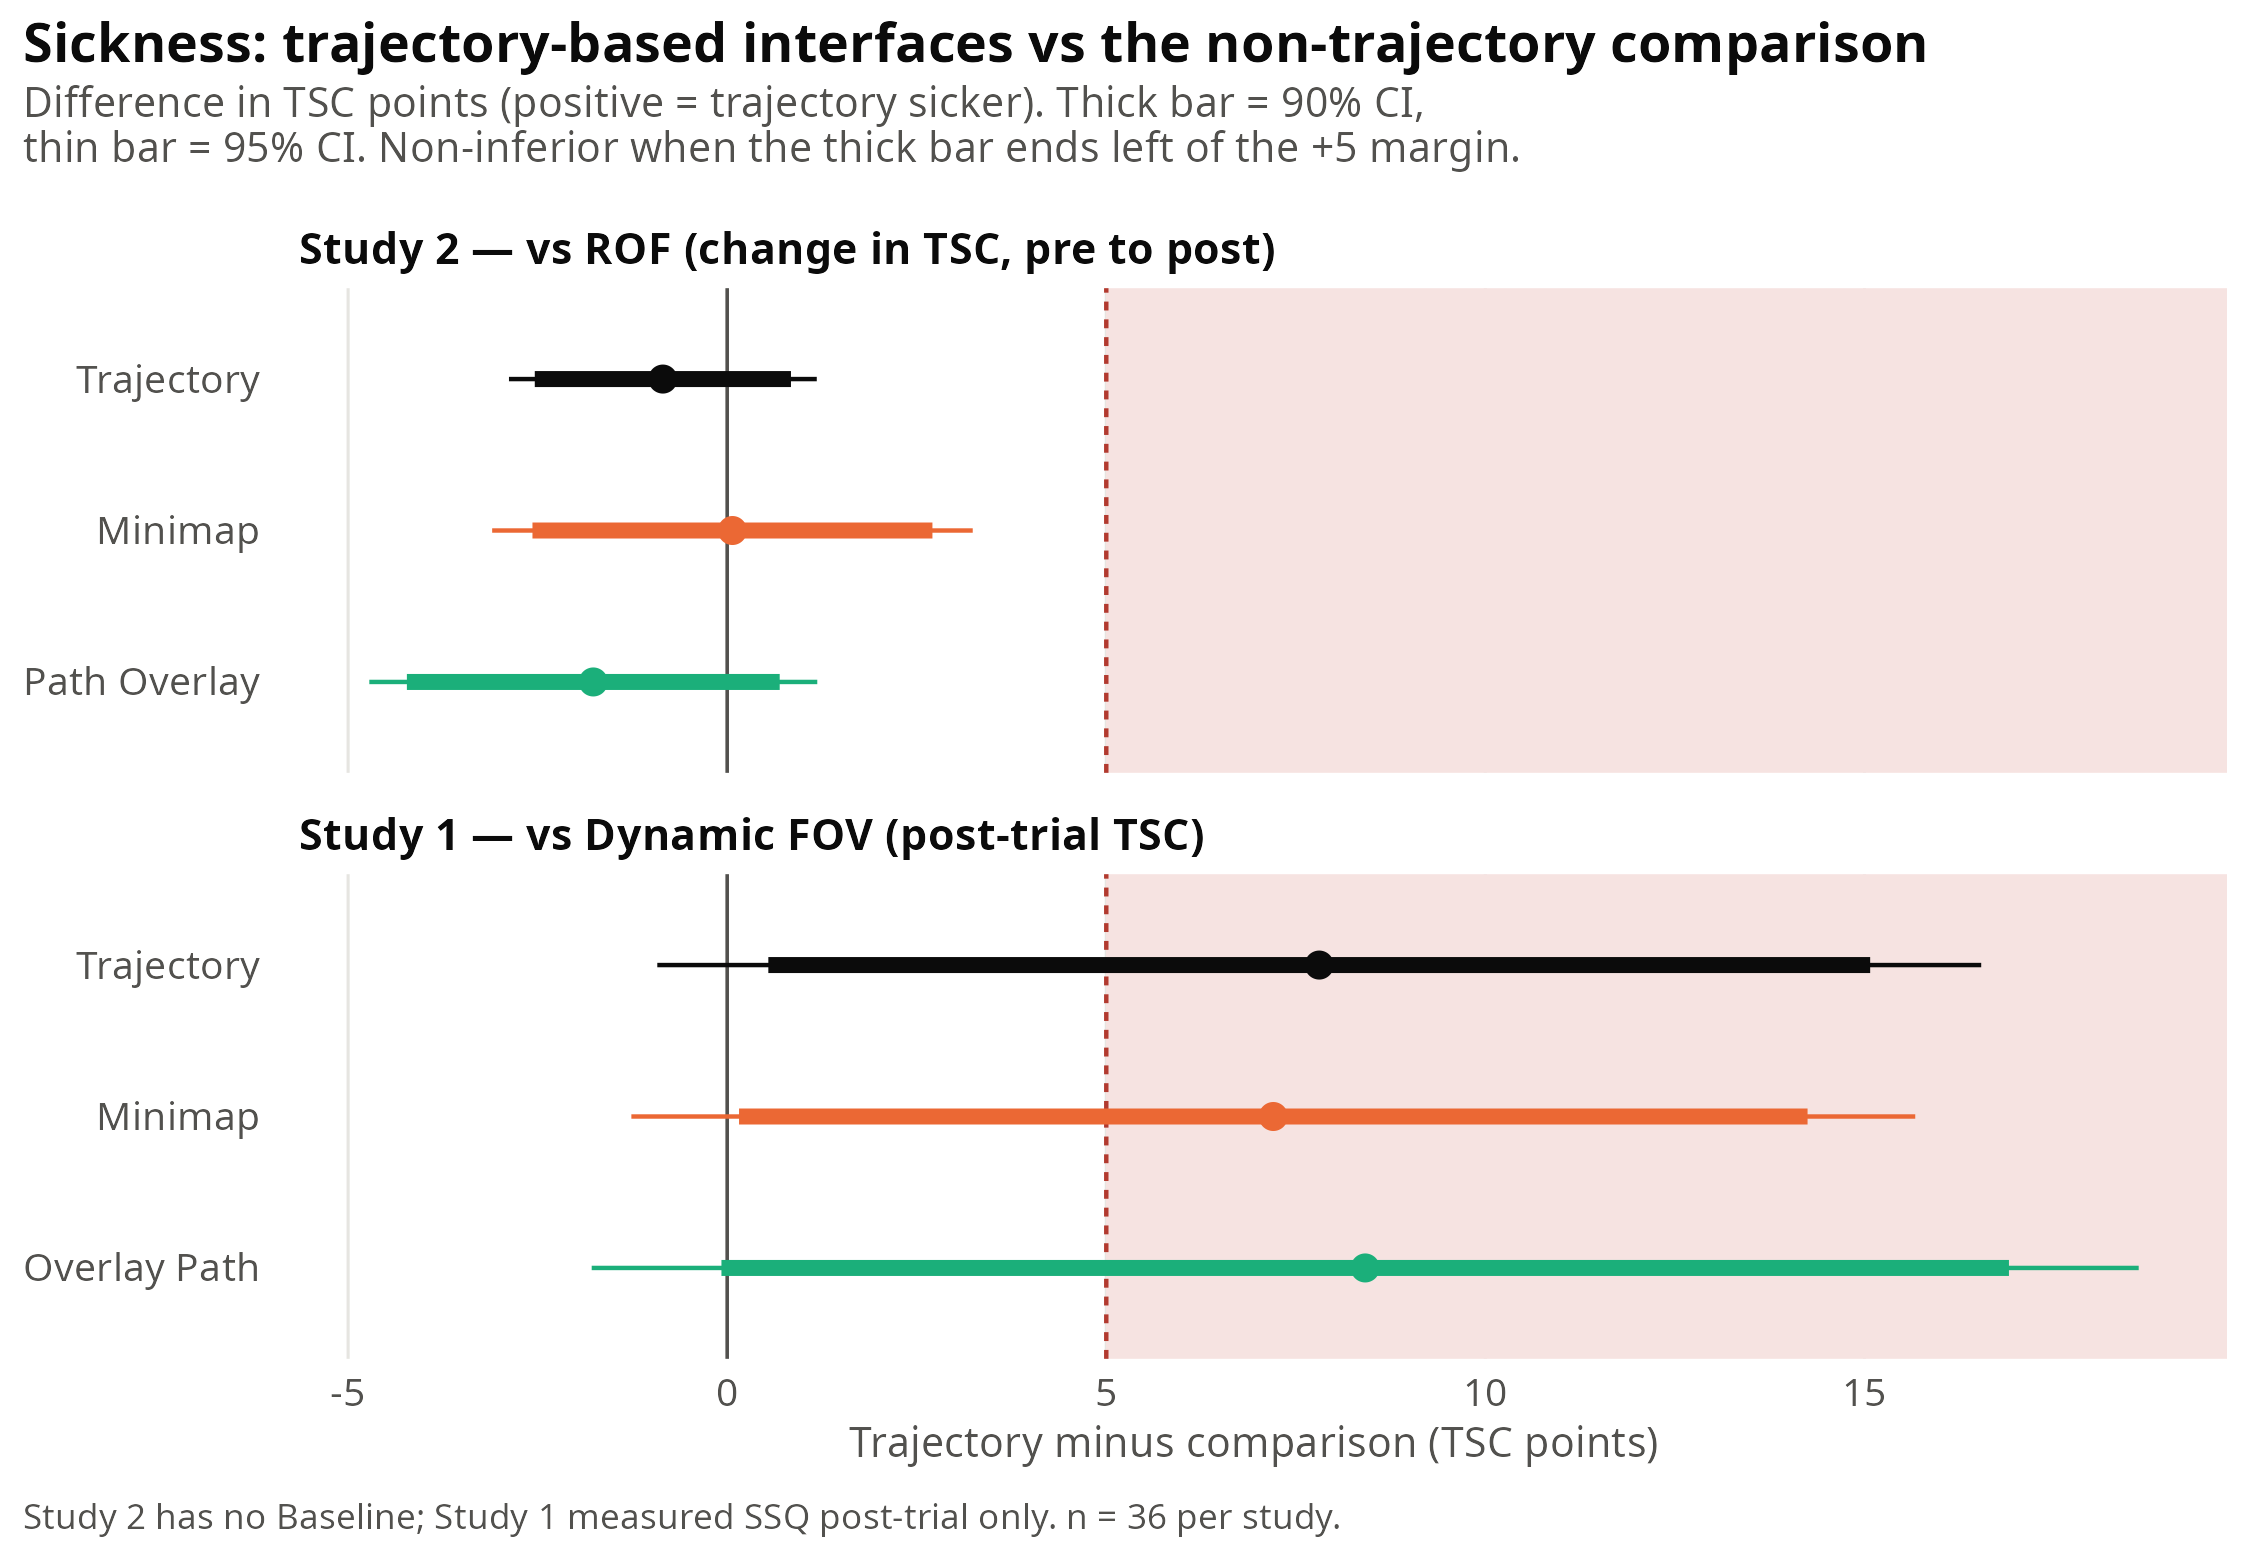
\includegraphics[width=0.8\textwidth]{figures/study2_noninferiority.png}
  \caption{Sickness difference between the trajectory-based interfaces and the
  non-trajectory comparison in each study. Thick bars show the 90\% CI and thin
  bars the 95\% CI; the dashed line marks the $+5$ TSC non-inferiority
  margin.}
  \label{fig:s2-ni}
\end{figure*}

\subsubsection{Presence}

Unlike in Study~1, \textbf{Presence did not differ between methods}
($F(1.84, 64.48) = 0.25$, $p = .758$); the effects of Video and Method $\times$
Video were also not significant. The trajectory-based interfaces scored 0.02
points lower than ROF (95\% CI [$-0.23$, 0.19]), and all three methods averaged
about 5.1 on the 7-point scale. Presence was unrelated to the increase in
sickness ($r = -.04$, $p = .82$). None of the three methods therefore showed
the Presence cost that Dynamic FOV showed in Study~1.

\subsubsection{Intrusiveness-Related Complaints}

\textbf{The trajectory-based interfaces did not receive fewer recorded
complaints than ROF} (Figure~\ref{fig:s2-complaints}). Thirteen participants
(36\%) complained about ROF, 7 (19\%) about Minimap, and 13 (36\%) about Overlay
Path. The mean within-participant difference was $+0.08$ (bootstrap 95\% CI
[$-0.08$, 0.26]; exact one-sided $p = .247$), and Minimap alone did not differ
significantly from ROF (exact McNemar test, Holm-corrected $p = .36$). Instead,
the complaints differed in \emph{kind}:

\paragraph{ROF.}
Flicker and visual clutter were ROF's main problem (9 participants, compared
with 1 for Minimap and none for Overlay Path), e.g., ``too many motion vectors''
or white streaks that caused glare. Opinions on occlusion were split (7 for, 7 against). At the same time,
ROF was the method most often praised for realism (13), for example for
creating a ``wind effect'' or blending with the surrounding scene.

\paragraph{Minimap.}
No participant said that the Minimap blocked the scene, and 13 praised it for
keeping the view clear; 10 valued its preview of the route. Attention was the
main issue: 5 participants found it distracting, while 5 others said they did
not notice it or forgot to look at it.

\paragraph{Overlay Path.}
Anticipating upcoming turns was the most frequently cited advantage of any
method in the study (17 participants), and 11 found the Overlay Path realistic.
However, it also received the most distraction complaints (8), and 6
participants said that it was too large or blocked the scene.

The comparison depended on which complaint types were counted. Excluding
distraction, where Overlay Path received the most complaints, produced a
significant difference ($p = .012$), whereas excluding visual noise, ROF's main
problem, removed any difference ($p = .70$). The interviews were coded by one
researcher and inter-rater reliability has not been assessed, so we treat this
analysis as exploratory.
% TODO: update this paragraph if a second coder is added
% (scripts/study2_trajectory.R reports agreement automatically).

\begin{figure*}[t]
  \centering
  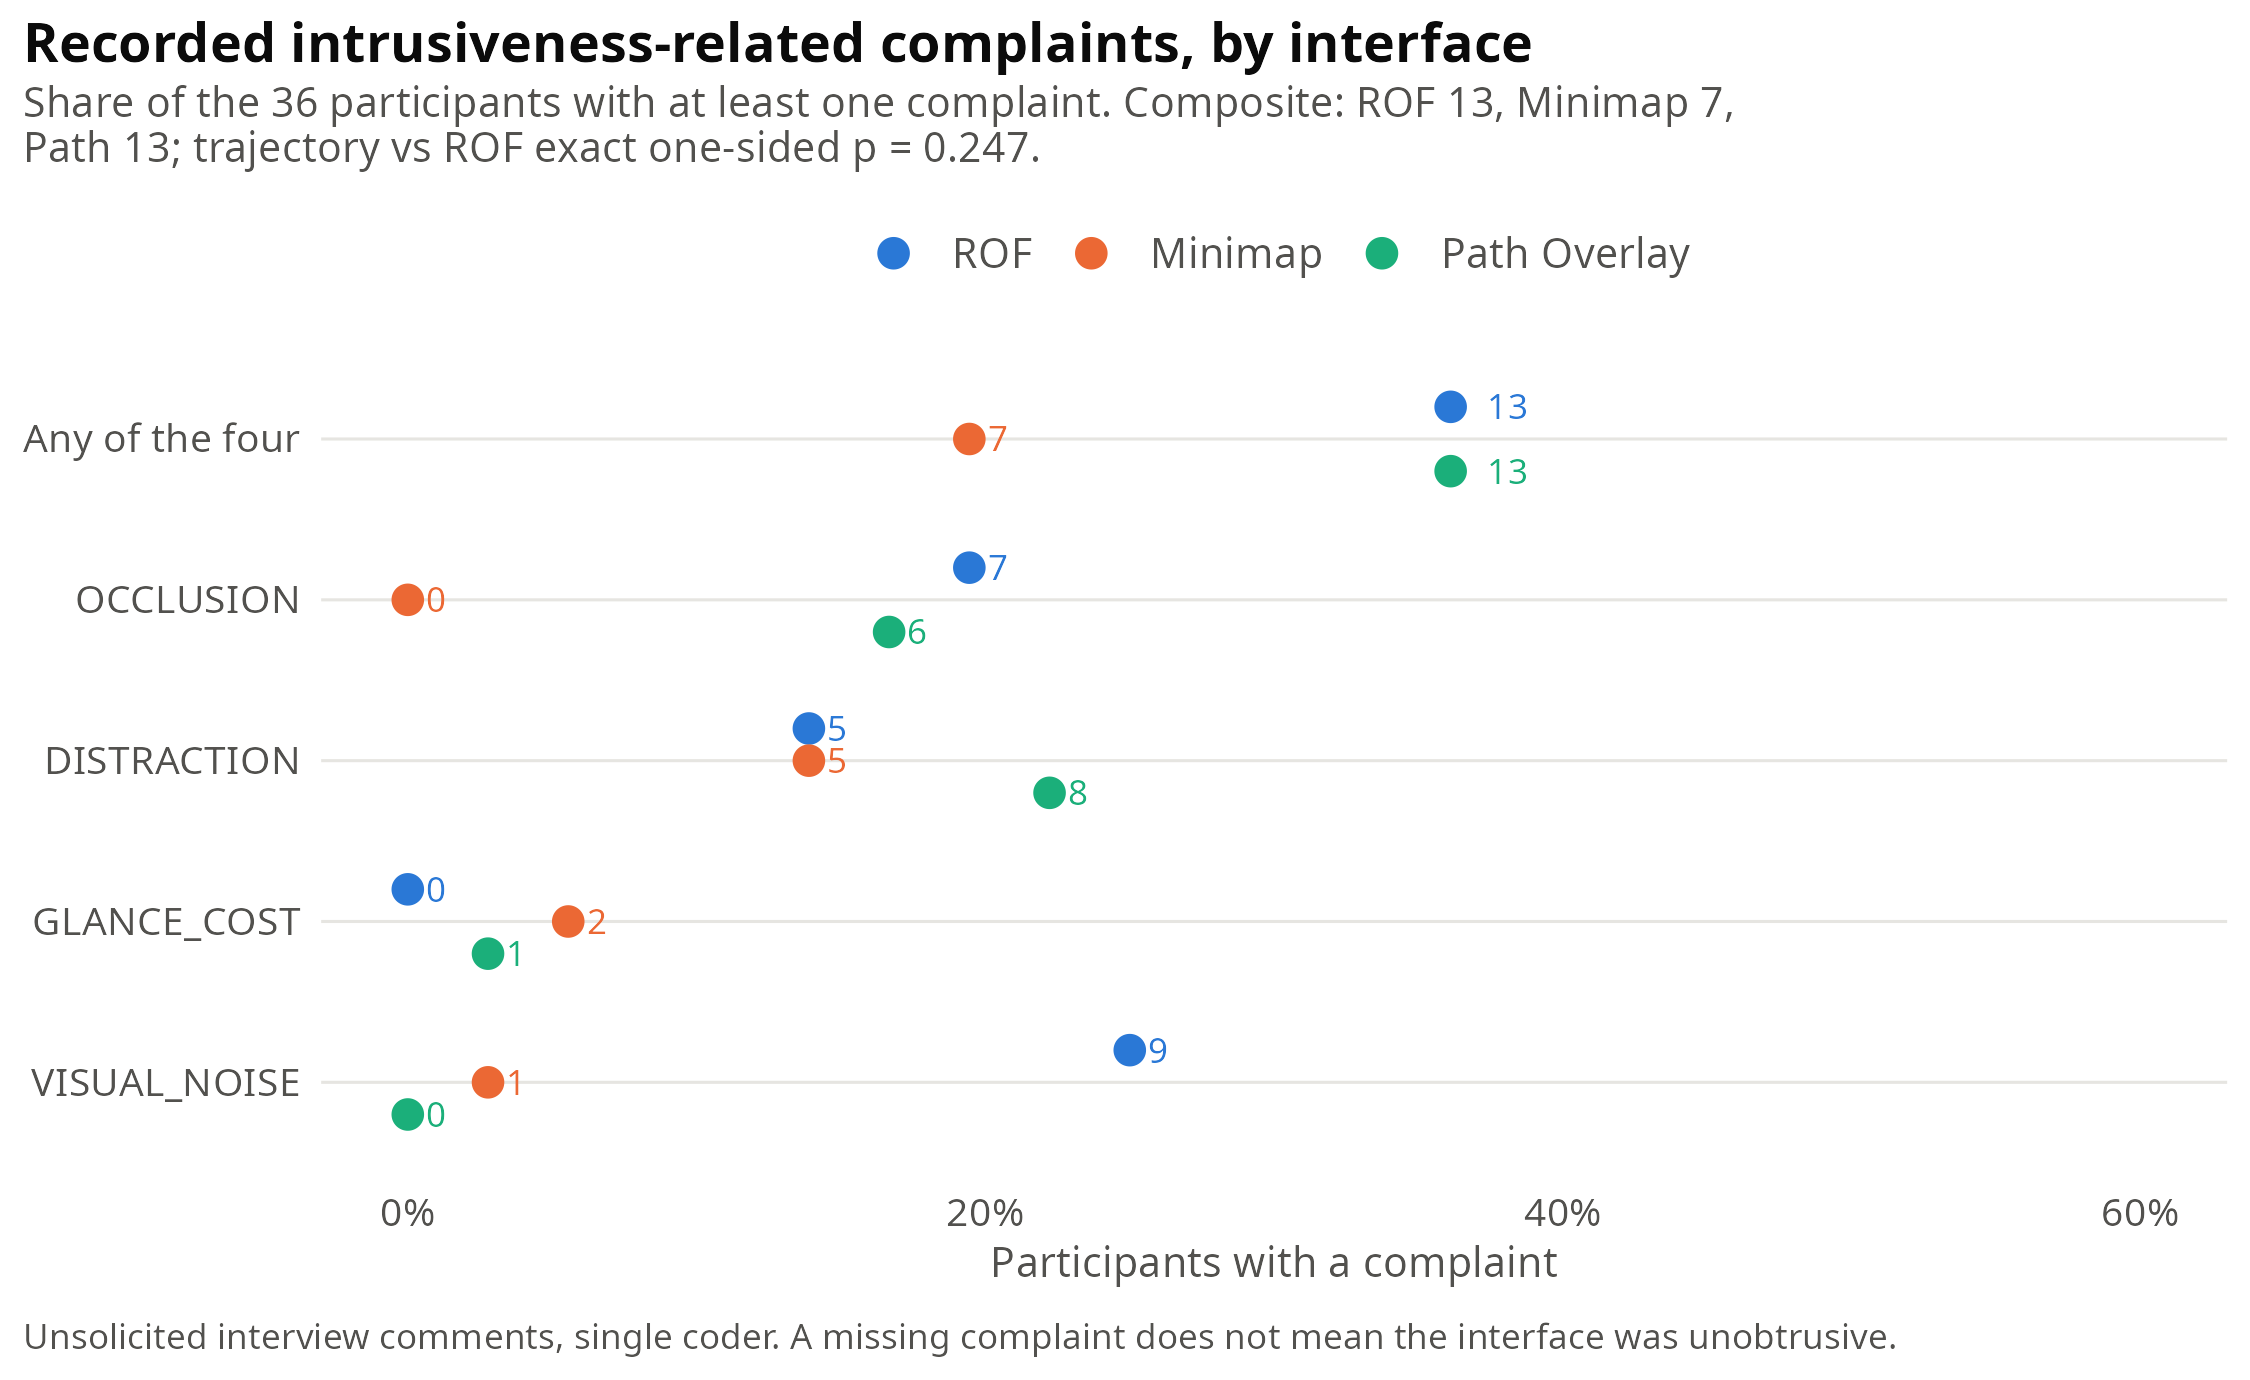
\includegraphics[width=0.8\textwidth]{figures/study2_complaints.png}
  \caption{Participants who made at least one recorded intrusiveness-related
  complaint about each method, overall (``any of the four'') and by complaint
  type. Counts are out of 36 participants.}
  \label{fig:s2-complaints}
\end{figure*}

\subsubsection{Preference Ranking}

Unlike in Study~1, all 36 participants provided a complete ranking
(Table~\ref{tab:s2-rank}). \textbf{No method was preferred overall}: the
rankings did not differ (Friedman $\chi^2(2) = 0.72$, $p = .697$), and
participants barely agreed with one another (Kendall's $W = .010$). ROF was
ranked last by 16 participants (44\%, 95\% CI [28, 62]), which was not more
often than expected by chance ($p = .11$). In the Plackett--Luce model, each
trajectory-based interface had an estimated probability of .36 of being ranked
first, compared with .27 for ROF, but this difference was not significant
(worth ratio 1.34, 95\% CI [0.78, 2.32], $p = .28$).

The secondary questions showed the same picture. Of the 21 participants who
named the method that best reduced their sickness, 8 chose ROF, 7 Minimap,
and 6 Overlay Path; of the 26 who named the most realistic method, 11 chose
ROF, 7 Minimap, and 8 Overlay Path.

When explaining their first choice, 86\% of participants referred to interface
experience, such as occlusion, distraction, or route anticipation, whereas only
19\% referred to sickness and 25\% to realism. \textbf{Participants' sense of
``balance'' therefore rested mainly on how each interface fit into the viewing
experience}, rather than on perceived sickness reduction.

\begin{table}[t]
  \caption{Preference ranking in Study~2 ($n = 36$). Lower mean rank indicates
  stronger preference. Borda score: 2 points for first place, 1 for second.}
  \label{tab:s2-rank}
  \centering
  \footnotesize
  \begin{tabular}{lcccc}
    \toprule
    \textbf{Method} & \textbf{Mean rank} & \textbf{Borda} & \textbf{First} & \textbf{Last} \\
    \midrule
    Overlay Path & \textbf{1.92} & \textbf{39} & \textbf{13} & \textbf{10} \\
    Minimap      & 1.97 & 37 & 11 & \textbf{10} \\
    ROF          & 2.11 & 32 & 12 & 16 \\
    \bottomrule
  \end{tabular}
\end{table}

\begin{table*}[t]
  \caption{Integration of quantitative and qualitative findings in Study~2.
  Interview counts are numbers of participants (out of 36).}
  \label{tab:s2-integration}
  \centering
  \footnotesize
  \begin{tabularx}{\textwidth}{lXX}
    \toprule
    \textbf{Method} & \textbf{Quantitative result} & \textbf{Interview feedback} \\
    \midrule
    Minimap      & TSC increased by 9.07; non-inferior to ROF (upper limit 2.71). Presence 5.12. &
                   Fewest intrusiveness-related complaints (7). Never described as blocking the scene; route preview valued (10). Some found it distracting (5) or forgot to look at it (5). \\
    Overlay Path & Numerically smallest TSC increase (7.24); non-inferior to ROF (upper limit 0.69). Presence 5.04. &
                   Most-cited advantage in the study: anticipating turns (17); seen as realistic (11). Most distraction complaints (8); too large or blocking the scene (6). \\
    ROF          & TSC increased by 9.00. Presence 5.10. &
                   Most often praised for realism (13), e.g., a ``wind effect''. Most complaints about flicker and visual clutter (9). Ranked last most often (16). \\
    \bottomrule
  \end{tabularx}
\end{table*}

\subsubsection{Study 2 Summary}

Table~\ref{tab:s2-integration} combines the quantitative and qualitative
results. Study~2 shows that \textbf{the trajectory-based interfaces were
non-inferior to ROF in measured VIMS}: sickness increased by a similar amount
under all three methods, and the data rule out the trajectory-based interfaces
being more than 0.84 TSC points worse than ROF on average. \textbf{Presence was
equally high for all three methods.} The data did \emph{not} show that the
trajectory-based interfaces were less intrusive: they drew about as many
recorded complaints as ROF, but of a different kind. ROF was criticized for
flicker, Overlay Path for distraction and occlusion, and Minimap drew the fewest
complaints. Participants did not agree on a single most balanced method; their
rankings followed these trade-offs rather than perceived sickness reduction.

These results have three limitations. First, Study~2 had no Baseline, so it
cannot show that any method reduced VIMS relative to unmodified video. Second,
sickness was mild (post-trial TSC 16.6--18.9, compared with 48.3--71.6 in
Study~1), which may have left little room for the methods to differ. Third,
the complaint analysis relies on unprompted comments coded by one researcher.

\section{Discussion}
\section{Conclusion}
%\bibliographystyle{abbrv}
\bibliographystyle{abbrv-doi}
%\bibliographystyle{abbrv-doi-narrow}
%\bibliographystyle{abbrv-doi-hyperref}
%\bibliographystyle{abbrv-doi-hyperref-narrow}

\bibliography{References}
\end{document}
